\documentclass[useAMS,usenatbib,referee]{biom}

\usepackage{graphicx,epsfig,amssymb,amsmath,bm,bbm,natbib,xcolor}
\usepackage{Sweave,hyperref}
\usepackage[colorinlistoftodos,linecolor=gray,backgroundcolor=white]{todonotes}   % to annotate text

% new command definitions
%\newtheorem{exercise}{Exercise}[chapter]
%\newtheorem{example}{Example}[chapter]
\newcommand{\ol}[1]{\overline{#1}}
\newcommand{\D}{\displaystyle}
\newcommand{\T}{\textstyle}
\newcommand{\s}{\scriptstyle}
\newcommand{\mc}[1]{\mathcal{#1}}
\newcommand{\bex}{\begin{exercise}}
\newcommand{\eex}{\end{exercise}}
\newcommand{\beg}{\begin{example}}
\newcommand{\eeg}{\end{example}}
\newcommand{\schist}[1]{\mbox{\tiny{#1}}}
\newcommand{\chist}[1]{\mbox{\scriptsize{#1}}}
\newcommand{\agemo}[1]{\mbox{$\underline{\omega}_{\/\downarrow #1}$}}
\newcommand{\ul}[1]{\mbox{$\underline{#1}$}}
\newcommand{\wh}[1]{\mbox{$\widehat{#1}$}}
\newcommand{\bv}{\begin{verbatim}}
\newcommand{\ev}{\end{verbatim}}
\newcommand{\bi}{\begin{itemize}}
\newcommand{\ei}{\end{itemize}}
\newcommand{\bfig}{\begin{figure}}
\newcommand{\efig}{\end{figure}}
\newcommand{\pref}[1]{\protect\ref{#1}}
\newcommand{\plab}[1]{\protect\label{#1}}
\newcommand{\be}{\begin{eqnarray}}
\newcommand{\bes}{\begin{eqnarray*}}
\newcommand{\ee}{\end{eqnarray}}
\newcommand{\ees}{\end{eqnarray*}}
\newcommand{\bo}[1]{\bf #1}
\newcommand{\bmt}[1]{\mbox{\boldmath $#1$}}
\newcommand{\tm}[1]{\mbox{\tiny{$#1$}}}
\newcommand{\vc}[2]{\mbox{$ \left[ \begin{array}{c} #1\\ \vdots \\ #2 
 \end{array} \right] $}}
\newcommand{\mt}[4]{\mbox{$ \left[ \begin{array}{c,c,c} #1 & \cdots & #2\\ 
 \vdots & \ddots & \vdots\\ #3 & \cdots & #4 \end{array} \right] $}}

\Sconcordance{concordance:paper.tex:paper.Rnw:%
1 4 1 1 0 81 1}

\bibliographystyle{chicago}


\title[2D or not 2D?]{Distance sampling detection functions: 2D or not 2D?}
\author{D.L. Borchers $^{*}$\email{dlb@st-andrews.ac.uk} \\
   Centre for Research into Ecological and Environmental Modelling, The Observatory \\
   Buchanan Gardens, University of St Andrews, Fife, KY16 9LZ, Scotland
   \and 
   M.J. Cox \\
   Australian Antarctic Division, Channel Highway Kingston TAS 7050,  Australia
   }

\begin{document}

\date{{\it Received XXXXX} 2014. {\it Revised XXXXX} 2014.  {\it
Accepted XXXXX} 2014.}

\pagerange{\pageref{firstpage}--\pageref{lastpage}}
\volume{??}
\pubyear{XXXX}
\artmonth{XXXXX}

\doi{10.1111/???}

\begin{abstract}
Conventional distance sampling (CDS) methods assume that animals are uniformly distributed in the vicinity of lines or points. But when animals move in response to observers before detection, or when lines or points are not located randomly, this assumption may fail. By formulating distance sampling models as survival models, we show that using time to first detection in addition to perpendicular distance (line transect surveys) or radial distance (point transect surveys) allows estimation of detection probability, and hence density, when animal distribution in the vicinity of lines or points is not uniform and is unknown. We also show that times to detection can provide information about failure of the CDS assumption that detection probability is 1 at distance zero. We obtain a maximum likelihood estimator of line transect survey detection probability and effective strip half-width using times to detection, and we investigate its properties by simulation in situations where animals are nonuniformly distributed and their distribution is unknown. The estimator is found to perform well when detection probability at distance zero is 1. It allows unbiased estimates of density to be obtained in this case from surveys in which there has been responsive movement prior to animals coming within detectable range. When responsive movement continues within detectable range, estimates may be biased but are likely less biased than estimates from methods that assuming no responsive movement. We illustrate by estimating primate density from a line transect survey in which animals are known to avoid the transect line, and a shipboard survey of dolphins that are attracted to it.
\end{abstract}

\label{firstpage}

\begin{keywords}
$g(0)=1$, line transect, point transect, removal method, responsive movement, survival analysis
\end{keywords}

\maketitle

\section{Introduction\label{intro}}

There are two main distance sampling methods: line transects and point transects. On line transect surveys observers traverse lines and record the perpendicular distances from the line to detected individuals, while on point transect surveys observers survey from points and record the radial distances to detected individuals. Observers may also record the locations in the plane of detected individuals, and other covariates. See \cite{Marques+al:10} and \cite{Buckland+al:01} for an overview of distance sampling methods.

Two key assumptions of distance sampling are (i) that the distribution of distances from samplers (lines or points) to individuals in the vicinity of the samplers is known (usually assumed uniform for line transects and triangular for point transects) and (ii) that detection of individuals at distance zero is certain \citep{Buckland+al:01}. Assumption (ii) is referred to as the ``$g(0)=1$'' assumption in distance sampling literature, where $g(x)$ is the probability of detecting an individual that is at perpendicular distance $x$ in the case of line transects, and radial distance $x$ in the case of point transects. In this paper we use $p(x)$ rather than $g(x)$ for the detection probability function.

We are interested in developing methods that do not require assumption (i) in particular, because on some surveys it may not be possible to meet this assumption. There are two main circumstances in which this is the case. The first is when samplers (lines or points) cannot be placed randomly, as may be the case in a jungle where observers are restricted to moving along paths, and we consider a visual line transect survey of primates where this was the case. The second is where animals move in response to an observer prior to being detected, and we consider a shipboard dolphin survey in which this was the case. %(Assumption (i) is often a bit weaker than above, being that perpendicular distances are uniformly distributed in the case of line transects, and have a triangular distribution in the case of point transects - both of which are true when individuals are uniformly distributed in space.) Should either assumption be violated, abundance estimates may be biased. 

%Distance sampling surveys do not routinely record times to detection, although in the case of line transect surveys forward distances to detections are sometimes recorded and radial distance and angle from transect line are frequently recorded on shipboard surveys. Times to detection can be obtained from these if observer speed is known. Times to detection although they are easy to obtain on many distance sampling surveys. We consider the utility of such data here. 
We show below that distance sampling methods that use times to detection do not require assumption (i) and that these methods are kinds of removal methods \citep[see][, Chapters 7 and 5, respectively, for an overview of removal methods]{Seber:82, Borchers+al:02}. And since removal methods require neither assumption (i) nor assumption (ii), we investigate the extent to which use of times to detection allows assumption (ii) to be relaxed as well. 

While times to detection are not used by current distance sampling methods, something akin to them were used in some old line transect survey models and we briefly review the reasons that their use was abandoned. But first we consider removal methods as these provide some insights for distance sampling surveys with time to detection.%, and the link with removal methods is useful for interpreting some aspects of the distance sampling models that we develop below.

\subsection{Removal models as survival models\label{sec:removal.surv}}

Removal methods involve repeated sampling and removing animals from a population when they are detected or captured. (We refer to detection, capture and removal as ``detection'' henceforth.) In the simplest model, all animals are assumed to be equally detectable and sampling effort is assumed to be the same on each occasion. %Variants include parameterising detection probability as a function of effort and inclusion of sex (for the ``change-in-ratio'' method) as an individual-level covariate. 

We can formulate a removal method with occasions $1,\ldots,T$ as a discrete time survival process with constant detection probability $p$ and an unknown number of right-censored individuals. In this case the ``survivor function'' (the probability of not being detected by occasion $(t-1)\in \{1,\ldots,(T-1)\}$) is $S(t-1)=(1-p)^{t-1}$ and the probability of being detected at time (occasion) $t\in \{1,\ldots,T\}$ is $f(t)=S(t-1)p$ (i.e. $t$ has a geometric distribution). The likelihood for the abundance $N$ and detection probability $p$, given that $n_t$ individuals were detected at time $t$ ($t=1,\ldots,T$) is multinomial: ${\cal L}(N,p)
=\left(\frac{N!}{(N-n)!\prod_{t=1}^Tn_t!}\right) S(T)^{N-n}\prod_{i=1}^{n}S(t_i-1)p$, where $n=\sum_t n_t$ and $N-n$ is the unknown number of censored survival times. The focus of inference is the number of censored times. Although it is not usually formulated as a discrete survival model, the simple removal method likelihood \citep[see Equation 5.4 on page 76 of][for example]{Borchers+al:02} is identical to the equation above. %The essential equivalence of a constant-hazard survival model and the simple (constant detection probability) removal model is visually apparent by noting that the removal method plot of expected cumulative removals against time is the same as the plot of expected number of survivors against time, but with the y-axis inverted.

The link between removal methods and distance sampling methods becomes apparent when we consider the continuous-time analogue of the discrete-time removal model -- which we now do. We start by considering a survey of duration $T$ with fixed hazard per unit time of detection, $h$. In this case the survivor function at time $t$ is $S(t;h)=\exp\{-\int_0^th\;du\}=\exp\{-th\}$ and the probability density function (pdf) of the $n$ detection times, given detection, is $f(\bmt{t}|\bmt{t}\leq T)=\prod_{i=1}^n\frac{S(t_i;h)h}{1-S(T;h)}$, where $\bmt{t}\leq T$ indicates that $t_1,\ldots,t_{n}$ are all less than or equal to $T$. Note that $1-S(T;h)$ is the probability of detection by time $T$, which we denote $p$. The corresponding likelihood function %(with unknown parameters $N$ and $h$) 
for the survey is ${\cal L}(N,h)=B\left(n;N,p\right)\prod_{i=1}^n\frac{S(t_i)h}{p}$, where $B\left(n;N,p\right)$ is a binomial probability mass function (pmf) with index $N$ and ``success'' probability $p$, evaluated at $n$.

Suppose now that in addition to the time that an individual has been at risk of detection ($t$), the detection hazard depends on a continuous individual random effect $x$ with pdf $\pi(x;{\bmt{\phi}})$ and parameter vector ${\bmt{\phi}}$. We assume that individuals' $x$s are independent draws from this distribution. The detection hazard is now $h(t,x;{\bmt{\beta}})$, where ${\bmt{\beta}}$ is a vector of unknown parameters, the survivor function is $S(t,x;{\bmt{\beta}})$, and detection probability, conditional on $x$ is $p(x;{\bmt{\beta}})=1-S(T,x;{\bmt{\beta}})=1-\exp\{-\int_0^Th(u,x;{\bmt{\beta}})du\}$. The mean detection probability in the population is $p_\cdot({\bmt{\beta}},{\bmt{\phi}})=E_x[p(x;{\bmt{\beta}},{\bmt{\phi}})]=\int\pi(u;{\bmt{\phi}})p(u;{\bmt{\beta}})du$, where integration is over the survey region. The likelihood function can now be written as
\be
{\cal L}(N,{\bmt{\beta}})
&=&
B\left(n;N,p_\cdot({\bmt{\beta}},{\bmt{\phi}})\right)
\prod_{i=1}^n
\pi(x_i|t_i\leq T)f(t_i|x_i,t_i\leq T) \nonumber \\
&=&
B\left(n;N,p_\cdot({\bmt{\beta}},{\bmt{\phi}})\right)
\prod_{i=1}^n
\frac{\pi(x_i;{\bmt{\phi}})p(x_i;{\bmt{\beta}})}{\int\pi(u;{\bmt{\phi}})p(u;{\bmt{\beta}})du}
\frac{S(t_i,x_i;{\bmt{\beta}})h(t_i,x_i;{\bmt{\beta}})}{p(x_i;{\bmt{\beta}})} 
\label{eq:DSremoval1} \\
&=&
{N \choose n}[1-p_\cdot({\bmt{\beta}},{\bmt{\phi}})]^{N-n}\prod_{i=1}^n \pi(x_i;{\bmt{\phi}})S(t_i,x_i;{\bmt{\beta}})h(t_i,x_i;{\bmt{\beta}})
\label{eq:DSremoval2}
\ee

\noindent
The term $[1-p_\cdot({\bmt{\beta}},{\bmt{\phi}})]^{N-n}$ is for the unknown number ($N-n$) of censored survival times.

\subsection{Distance sampling models as survival models\label{sec:DS.surv}}

Although they are traditionally treated as instantaneous surveys, distance sampling surveys seldom really are. An individual at (perpendicular or radial) distance $x$ is in view for some period (of length $T$ say), and at time $0\leq t\leq T$ it has some hazard $h(t,x;{\bmt{\beta}})$ of being detected. Detected individuals are effectively removed if the usual distance sampling protocol of recording only the locations of individuals when first detected, is used. In this case, one can consider a distance sampling survey to be a removal survey of the sort described immediately above, and hence also as a kind of survival model survey. 

Indeed, the conventional distance sampling full likelihood is identical to Equation~(\ref{eq:DSremoval1}) with the random effect $x$ being perpendicular distance (in the case of line transects) or radial distance (in the case of point transects), except that with distance sampling (a) the random effect distribution $\pi(x_i;{\bmt{\phi}})$ is treated as known, and (b) the term with detection times ($f(t_i|x_i,t_i\leq T)=S(t_i,x_i;{\bmt{\beta}})h(t_i,x_i;{\bmt{\beta}})/p(x_i;{\bmt{\beta}})$) is omitted - see \cite{Buckland+al:04}, Equation~(2.33) or \cite{Borchers+al:02}, Equation~(7.10). We are concerned in this paper with situations in which it is not reasonable to treat $\pi(x_i;{\bmt{\phi}})$ as known, and we show below that $f(t_i|x_i,t_i\leq T)$ is useful for estimating it.

Omitting $f(t_i|x_i,\bmt{t}\leq T)$ from distance sampling likelihoods reduces the data from two dimensions ($x$ and $t$) to one dimension ($x$) and as a result $\pi(x_i;{\bmt{\phi}})$ and $p(x_i;{\bmt{\beta}})$ are confounded: without $f(t_i|x_i,\bmt{t}\leq T)$ they appear only as a product in Equation~(\ref{eq:DSremoval1}). This begs the question ``Why are conventional distance sampling detection functions one dimensional?''. In the case of line transect surveys, the answer can be found in a landmark paper by \cite{Hayes+Buckland:83}.

%\subsection{Line transect surveys}

They considered line transect detection function models that included forward distances. (Using forward distance, $y$, is equivalent to using times to detection if observers move at constant speed, $v$, since $y=y_{max}-vt$ - see Figure~\ref{fig:ltT}.) %These models were formulated in terms of perpendicular and radial distance rather than perpendicular and forward distance, but it is straightforward to switch between the two. They key point is that they 
These are two-dimensional (2D) line transect detection function models (with forward distance $y$ as well as perpendicular distance, $x$) and the key question here is why 2D detection models were abandoned. 

\begin{figure}
\begin{center}
\caption{Line transect notation. The grey line is a transect line that starts on the left of the figure. The smiley face is individual $i$, located at perpendicular distance $x_i$ from the line and distance $l_i$ along the line. At time $\tau$ an observer (the dark circle) is a distance $l(\tau)$ along the line, moving at speed $v$ from left to right along the line. The dotted box is the window in which individuals can be detected by the observer at time $\tau$ and it moves with the observer. It extends a distance $w$ either side of the line and a distance $y_{max}$ ahead of the observer. Stationary individuals within $w$ of the line are in the window for a time $T$. In the figure, individual $i$ has been in view for a time $t_i$ and is at forward distance $y_i(t_i)$ ahead of the observer. When individual $i$ enters the window, it has time $t_i=0$ and  forward distance $y_i(0)=y_{max}$, and when it passes abeam of the observer, it has $t_i=T$ and $y_i(T)=0$. \label{fig:ltT}}
\vspace{12pt}
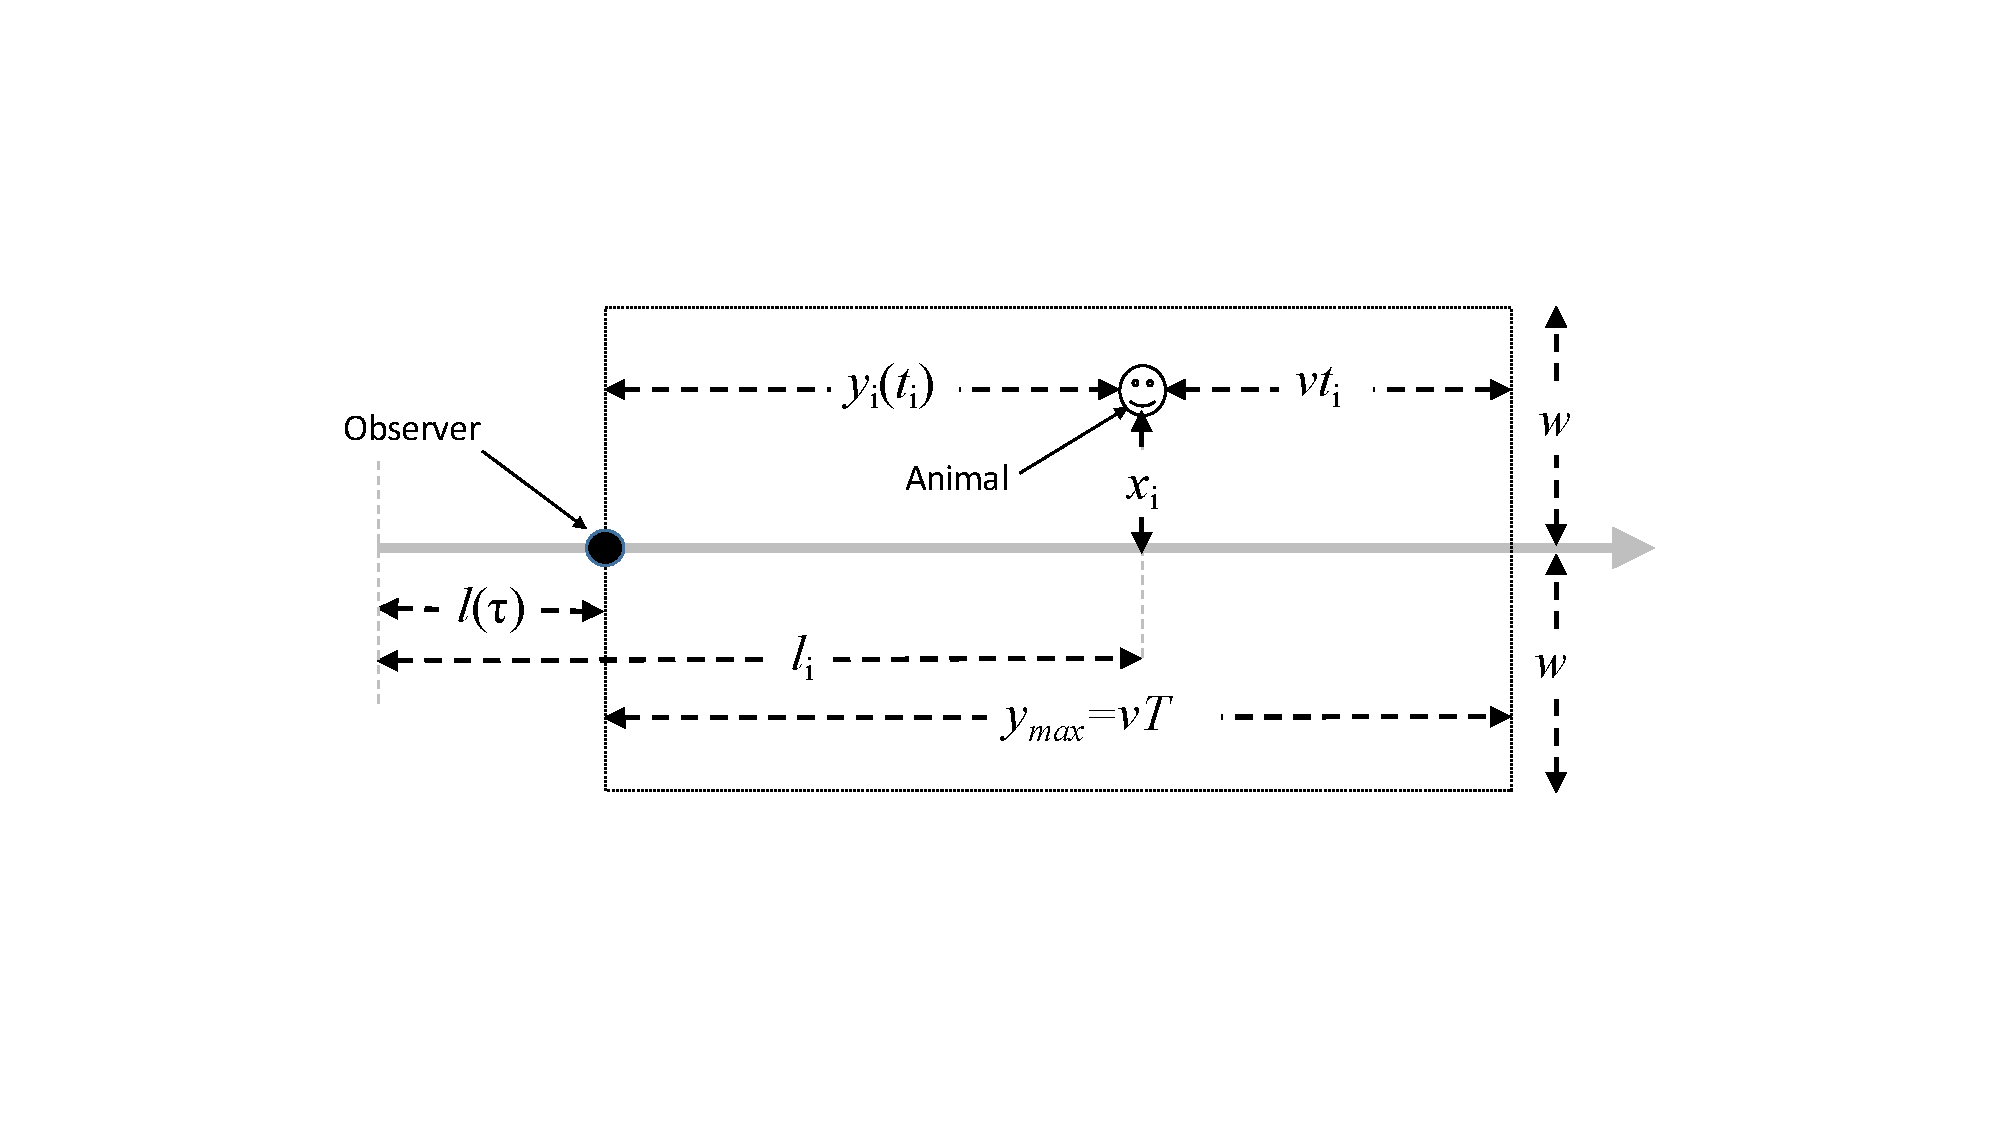
\includegraphics[width=15cm]{ltT.pdf}
\end{center}
\end{figure}


\citet{Hayes+Buckland:83} considered the 2D detection models of \cite{Hayne:49}, \cite{Eberhardt:78}, \cite{Burnham+Anderson:76} and \cite{Burnham:79}. %These are all based on rather restrictive assumptions about the detection process and i
% * <martinjamescox@gmail.com> 2016-05-20T05:36:39.816Z:
%
% > \cite{Burnham+Anderson:76} 
%
% changed ref
%
% ^.
In their examination of these models, \citet[][p 33]{Hayes+Buckland:83} conclude that ``none of the models appears to be founded upon realistic assumptions.'' They went on to develop a survival model for the detection process (although they did not call it a survival model)%, their model is a survival model just like that developed in Section~\ref{sec:removal.surv} above
, with a detection hazard that depends on forward and perpendicular distance.

%The model of \cite{Hayes+Buckland:83} used a hazard function, $k(r,x)$, formulated in terms of radial distance $r$ and perpendicular distance $x$, rather than time and perpendicular distance as in Section \ref{sec:removal.surv}, but it is straightforward to switch between the two formulations. Their 
The key conclusion of \cite{Hayes+Buckland:83} with regard to density estimators ($\hat{D}$) from 2D hazard models was (p39) ``We do not believe that the estimator $\hat{D}$ will be robust to the form arbitrarily chosen for [the hazard function] when observed radial distances are used for estimation.'' (The 2D models they considered used radial and perpendicular distances, rather than forward and perpendicular distances.) %\footnote{\cite{Hayes+Buckland:83} use $y$ for perpendicular distance; we use $x$. We have changed ``$k(r,y)$'' to ``$k(r,x)$'' in this quotation for consistency with our notation.} 
They went on to develop a new form of 1D (perpendicular distance only) detection function (the now well-known ``hazard rate'' form) based on their survival model, and showed that this form is obtained from a variety of forms for the hazard function. 

\cite{Hayes+Buckland:83} concluded that the weakness of the 2D models they looked at was that they were ``arbitrary'' and ``founded on unrealistic assumptions''. But other 2D distance sampling models had been used successfully before 1983 \citep[][for example]{Schweder:74} and have been used successfully since. Examples include \citep{Schweder:90}, \cite{Schweder+al:96}, \cite{Schweder+al:97}, \cite{Schweder+al:99}, \cite{Skaug+Schweder:99}, \cite{Okamura:03}, \cite{Skaug+al:04}, \cite{Okamura+al:03}, \cite{Okamura+al:06}, \cite{Okamura+al:12}, \cite{Borchers+al:13}, \cite{Langrock+al:13} and  \cite{Borchers+Langrock:ip}. These papers used a variety of more flexible hazard function forms than the models considered by \cite{Hayes+Buckland:83}, including models that allow $p(0)<1$. However, all of them concern individuals that become available and unavailable for detection stochastically while within detection range. %(In a survival context, this would be like subjects switching in and out of being succeptible to mortality, according to some stochastic process.). We are not aware of any line transect models other than those considered by \cite{Hayes+Buckland:83} that use 2D detection models without also modelling stochastic individual availability. 
In a similar vein, \cite{Solymos+al:13} and \cite{Amundson+al:14} developed models for point transect surveys that use times to detection, for individuals that are stochastically available. These discretise time and have no probability mechanism for dealing with time intervals of different lengths, or continuous time. We develop 2D distance sampling models without stochastic individual availability here, and apply them with one of the hazard models proposed by \cite{Hayes+Buckland:83} and two of the hazard models proposed by the authors listed above. The detection hazard formulation above also provides a mechanism for extending models like those of \cite{Solymos+al:13} and \cite{Amundson+al:14} to deal with continuous time and/or intervals of different lengths.

%\subsection{Point transect surveys}

%On line transect surveys, time to detection and forward distance are interchangeable so that once one is recorded the other contains no new information, but this is not the case on point transect surveys (because observers do not move), and hence time to detection may add new information on detection probability beyond that provided by angle and distance. To our knowledge, no models using time to detection have been proposed for point transect surveys to date, although 2D models that use angles in addition to the conventionally recorded radial distances to detections have been developed by \cite{Marques+al:10a}, \cite{Cox+al:11} and \cite{Arranz+al:14} to deal with non-uniform distribution of individuals. 

%However, although they do not say so explicitly, these methods rely on the detection function gradient and density gradient not being coincident in order to separate change in detection probability from change in density. If the gradients coincide, the use of data on angles in addition to distances does not allow change in density to be separated from change in detectability. To deal with this limitation, \cite{Marques+al:10a} and \cite{Arranz+al:14} assumed that detection probability does not depend on angle, but density might, while \cite{Cox+al:11} obtained independent information on the rate of change of detection probability with angle. Because time to detection data are survival data, and detection probability can be estimated from survival data alone, the addition of time to detection data does in principle allow change in density to be separated from change in detectability.

%Note that if time to detection is included in conventional point transect models (which use only radial distance to detection), one has a 2D point transect model (using radial distance and time). But if time to detection is added to the far less common version of point transect models that use detection angles as well as radial distances, one has a 3D point transect model. We focus primarily on line transect models in what follows.


\subsection{Detection probability at distance zero}

Conventional distance sampling methods assume that $p(0)=1$. One can build this into 2D detection function models by choosing an appropriate hazard function form - as did \cite{Hayes+Buckland:83}, for example. Or one can use a hazard function form that does not require the $p(0)=1$ assumption, as did \cite{Langrock+al:13}, for example. 

Thinking of distance sampling data as removal (or survival) data, one would expect that it is possible to estimate abundance without assuming that $p(0)=1$ - since no such assumption is required for estimation from removal method data. On the other hand, the simple (constant $p$) removal method performs poorly unless a relatively high proportion of the population is detected \citep[see][Table 7.3, for example]{Seber:82}, i.e., unless $S(T)$ is close to 1. So one might also expect poor performance from 2D distance sampling estimators unless $p(0)=p(x=0;{\bmt{\beta}})=1-S(t,x=0;{\bmt{\beta}})$ is close to 1. We consider this further below.



\section{Distance sampling likelihood\label{sec:DSlikelihood}}

%We focus on estimation of animal density within the covered region - the part of the survey region within some distance $w$ of the lines that observers traverse or the points at which they are located. We refer to the lines or points collectively as ``samplers''. 

%We do not address the question of how to model the 2D distribution of individuals beyond a distance $w$ from samplers. Times to detection will typically be uninformative about large-scale variation in density across the  survey region because the truncation distance ($w$) and the maximum distance observers can see ($y_{max}$) are both typically only a tiny fraction of the dimensions of the survey region or the length of transect lines. As will be shown below, times to detection can be informative about variation in density within a distance $w$ of samplers, and in the rare cases in which $w$ and $y_{max}$ are not small fractions of the survey region dimensions, times to detection may well be useful for modelling spatial variation across the survey region, but here we focus on inference within distance $w$ of samplers.

Distance sampling observations arise only within some maximum searched distance $w$ of samplers (lines or points) and conventional distance sampling estimators of density and abundance commonly use design-based methods for drawing inferences outside of this ``covered region'', while model-based methods of inference are used within the covered region. Model-based methods are required within the covered region because inclusion probabilities are unknown, are beyond the control of the surveyor, and are estimated on the basis of a model for the detection function (with some unknown parameters) whereas the probability of individuals being in the covered region can be determined by design. Here we are concerned with inference within the covered region.

On a line transect survey, the location of individual $i$ is conveniently expressed as $x_i$, its distance from the line, and $l_i$, its distance along the line (see Figure~\ref{fig:ltT}). An observer moves along the line at constant speed $v$, such that her location along the line at time $\tau$ is $l(\tau)$, with a window of half-width $w$ and length $y_{max}=vT$ moving with her. Each individual has its own time coordinate ($T_i$ for individual $i$) which is set to 0 when the observer is a distance $y_{max}$ short of $l_i$, and at time $T_i=t_i$ it is at forward distance $y_i(t_i)$ ahead of the observer (Figure~\ref{fig:ltT}). So for line transects, the observer-centric coordinates are $(x_i,y_i(t_i))$.

As with conventional line transect models, we assume that the probability of detecting individual $i$ at perpendicular distance $x_i$ from the line does not depend on its distance $l_i$ along the line. (One can add covariates to the detection hazard to allow it to vary with distance along line.) This implies that the detection hazard function depends on $x_i$ and time in view ($t_i$), but not on $l_i$, so that it can be written as $h(x_i,y_i(t_i))$ and the survivor function can be written as $S(t_i,x_i)$. (The time that individuals at the start of the line with $l_i<y_{max}$ are in view is less than $T$ and this should strictly be taken account of in the likelihood. This ``end effect'' is usually negligible.) In the case of point transects, both the observer and the animals are assumed to be stationary until detection, so that unless the detection hazard varies with time, it can be written simply as $h(x_i)$, where in this case $x_i$ is the radial distance of animal $i$ from the observer.
% * <martinjamescox@gmail.com> 2016-05-20T05:43:51.729Z:
%
% > radial
%
% prependicular? 
%
% ^.

\subsection{Conditional likelihood}

Inference within the covered region is conventionally based on the conditional likelihood, given detection of $n$ objects in the covered region, not the unconditional likelihood given above (which includes a binomial probability model for $n$). This is to avoid having to model the distribution outside of searched strips or circles \citep{Borchers+Burnham:04}. The conditional likelihood is Equation~(\ref{eq:DSremoval1}) without the leading binomial pdf term:
\be
{\cal L}({\bmt{\beta}}|n)&=&f_{x|n}({\bmt{x}}|n)f_{t|x}({\bf t}|\bmt{x},\bmt{t}\leq T) \nonumber \\
&=&
\left\{
\prod_{i=1}^n
\frac{\pi(x_i;{\bmt{\phi}})p(x_i;{\bmt{\beta}})}{\int\pi(u;{\bmt{\phi}})p(u;{\bmt{\beta}})du}
\right\}
\left\{
\prod_{i=1}^n
\frac{S(t_i,x_i;{\bmt{\beta}})h(t_i,x_i;{\bmt{\beta}})}{p(x_i;{\bmt{\beta}})} 
\right\}
\label{eq:cond.lik}
\ee
%\begin{eqnarray}
%\mathcal{L}_{cond}({\bmt{\phi}},{\bmt{\beta}})
%=f_{s|n}(\bmt{s}|n)f_{t|s}({\bf t}|\bmt{s}) 
%=
%\left\{\prod^{n}_{i=1} \frac{D(\bmt{s}_i)p(\bmt{s}_i)}{\int_{R^2}D(\bmt{s})p(\bmt{s})d\bmt{s}}\right\}
%\left\{\prod^{n}_{i=1}\frac{S(t_i,\bmt{s}_i)h(\bmt{x}(\bmt{s}_i,t_i))}{p(\bmt{s}_i)}\right\}
%\label{eq:cond.lik}.
%\end{eqnarray}
\noindent
where $\bmt{x}=(x_1,\ldots,x_n)$, $\bmt{t}=(t_1,\ldots,t_n)$ and $\bmt{t}\leq T$ indicates that all of $t_1,\ldots,t_n$ are less than or equal to $T$. Here $f_{x|n}({\bmt{x}}|n)$ is the conditional likelihood, but allowing a more general form for $\pi(x_i;{\bmt{\phi}})$ than is conventionally used. With CDS, uniform object density within $w$ of the observer is usually assumed, so that for line transects $\pi(x_i;{\bmt{\phi}})=C$ for some constant $C$, and $C$ cancels in $f_{x|n}({\bmt{x}}|n)$, leaving $\prod_i p(x_i)/\int p(x)dx$, which is the CDS conditional likelihood for line transects \citep[see][]{Buckland+al:01}. Similarly, with uniform object density for point transects $\pi(x_i;{\bmt{\phi}})\propto x_i$ \citep[see][]{Buckland+al:01} giving the CDS point transect conditional likelihood $\prod_i\left\{x_ip(x_i)/\int xp(x)dx\right\}$. It is standard practice with distance sampling inference not to use times to detection and so CDS likelihoods do not involve the component $f_{t|x}({\bf t}|{\bmt{x}})$. We do include times to detection and $f_{t|x}({\bf t}|{\bmt{x}})$, and it is this that enables us to deal with unknown $\pi(x_i;{\bmt{\phi}})$, responsive movement prior to detection, and to some extent uncertain detection at distance zero.



\subsection{CDF and PDF of detection times}

The shape of the pdf of detection time $t$ at distance zero, given $t\leq T$, i.e. $f_{t|x}(t|x,t\leq T)=\frac{S(t_i,x_i)h(t_i,x_i)}{p(x_i}$ (omitting $\bmt{\beta}$ for brevity), turns out to be somewhat informative about $p(0)$. If $p(0)=1$ then $f_{t|x}(t|0,t\leq T)$ must approach zero as $t\rightarrow T$, as in this case no animals at distance $x=0$ survive detection beyond $T$ (forward distances $y<0$ in the case of line transects). As a result there will be no detections at, or very close to $(x=0,t=T)$ (or to $(x=0,y=0)$ for line transects). This in turn means that $f_{t|x}(t|0,t\leq T)$ must have a mode at $t\leq T$ ($y>0$). Conversely, if it does not then this implies that $p(0)$ is less than 1. 

The cumulative distribution function (CDF) of $t$ is the scaled probability that an object at $x$ survives detection up to time $t$: $F_{t|x}(t|x)=S(t,x)/\int_0^T S(t,x)dt$. This is analogous to the removal method CDF and as with removal methods, when $F_{t|x}(t=T|x)$ is not close to 1 (i.e. when, by the end of the period in which animals are at risk of removal/detection, not a large fraction of the available population has been removed/detected), estimation of the proportion of the available population that has been removed/detected (and specifically $p(0)=F_{t|s}(t=T|0)$ in the present context), can not be done reliably.

The mean pdf of $t$, given detection, is useful for visually assessing goodness of fit in the $t$ dimension. For line transects this is $E_x[f_{t|x}(t|x)]=\int_x^w f_{t|x}(t|x,t\leq T))\pi(x;\bmt{\phi})dx$ where $f_{t|x}(t|x,t\leq T)$ is the pdf of $t$ given distance $x$ and detection. 


\section{Detection hazards and perpendicular distance distributions}

We now focus on line transect surveys. Although our models are formulated above in terms of detection times, when observers move at constant speed it is convenient to work in terms of forward detection distances ($y$) rather than times, which we do henceforth. We use one of the hazard forms (model $h_{HB}$ below) proposed by \cite{Hayes+Buckland:83} as well as the exponential power and inverse power hazard models that were used by \cite{Langrock+al:13} ($h_{EP}$ and $h_{IP}$). We also generalise $h_{HB}$ to allow $p(0)<1$ (hazard $h_{HB2}$) and the latter two  to allow separate scale parameters for $x$ and $y$ (models $h_{EP2}$ and $h_{IP2}$). The models are as follows ($\beta_j>0$ for all $j$):
\begin{eqnarray}
h_{HB}(\boldsymbol{x};\boldsymbol{\beta})=\beta_1 (x^2+y^2)^{-(\beta_2+2)/2}& &
%h_{HB2}(x;\boldsymbol{\beta})&=&\beta_0 y(x^2+y^2)^{-(\beta_1+3)/2}\;\;\;\;\;\;\;\;\;\;(\beta_1,\beta_2>0) \nonumber \\
h_{HB2}(\boldsymbol{x};\boldsymbol{\beta})=\beta_1 (x^2+(y+\beta_3)^2)^{-(\beta_2+2)/2} \nonumber \\
h_{IP}(\boldsymbol{x};\boldsymbol{\beta})=\beta_1\left\{1+\left(\frac{x}{\beta_2}\right)^2+\left(\frac{y}{\beta_2}\right)^2\right\}^{-(\beta_3+1)/2}& &
h_{EP}(\boldsymbol{x};\boldsymbol{\beta})=\beta_1\exp\left\{\left(\frac{x}{\beta_2}\right)^{\beta_3}+\left(\frac{y}{\beta_2}\right)^{\beta_3}\right\} \nonumber \\
h_{IP2}(\boldsymbol{x};\boldsymbol{\beta})=\beta_1\left\{1+\left(\frac{x}{\beta_2}\right)^2+\left(\frac{y}{\beta_4}\right)^2\right\}^{-(\beta_3+1)/2}& &
h_{EP2}(\boldsymbol{x};\boldsymbol{\beta})=\beta_1\exp\left\{\left(\frac{x}{\beta_2}\right)^{\beta_3}+\left(\frac{y}{\beta_4}\right)^{\beta_3}\right\} \nonumber
\end{eqnarray}
The hazard $h_{HB}$ has $p(0)=1$, whereas the other hazards allow $p(0)<1$. We use slightly different forms for $h_{EP}$ and $h_{IP}$ than do \cite{Langrock+al:13}, in that we allow $\beta_1$ to be greater than 1 (because our hazard functions are rates, not probabilities). 

As is done with CDS methods, we use the absolute value of perpendicular distance so that $x\geq 0$, and we right-truncate $x$ at a distance $w$ from the transect line. We consider these forms for $\pi(x;\boldsymbol{\phi})$ $(\phi_1>0;-\infty\leq\phi_2\leq\infty)$:
\begin{eqnarray}
\pi_{U}(x;\boldsymbol{\phi})=\frac{1}{w}& &
\pi_{HN}(x;\boldsymbol{\phi})=e^{-\frac{x^2}{2\phi_1^2}}\left\{\int_0^we^{-\frac{x^2}{2\phi_1^2}}dx\right\}^{-1} \nonumber \\
\pi_{N}(x;\boldsymbol{\phi})=e^{-\frac{(x-\phi_2)^2}{2\phi_1^2}}\left\{\int_0^we^{-\frac{(x-\phi_2)^2}{2\phi_1^2}}dx\right\}^{-1}& &
\pi_{CN}(x;\boldsymbol{\phi})=\left\{1-e^{-\frac{x^2}{2\phi_1^2}}\right\}\left\{w-\int_0^we^{-\frac{x^2}{2\phi_1^2}}dx\right\}^{-1} \nonumber 
\end{eqnarray}
Model $\pi_{U}$ corresponds to no responsive movement,  $\pi_{HN}$ allows for attraction to the transect line, $\pi_{CN}$ for avoidance and $\pi_{N}$ for attraction or avoidance.

\section{Model selection, diagnostics and interval estimation}

The focus of inference is the inclusion probability in the covered region and the key quantity for this in the case of line transects is the effective strip half-width, defined as $\tilde{w}=\left(w\int_0^w p(x)\pi(x)dx\right)$, where $p(x)=1-S(T,x)$ and $T$ is the maximum time animals are within detectable range. (The inclusion probability is $\int_0^L2\tilde{w}dl/(2wL)=\tilde{w}/w$, where integration is along the transect and $L$ is the total transect length.) The variance-covariance matrix of model parameters is estimated using the inverse Hessian matrix obtained by maximising the conditional likelihood Equation~(\ref{eq:cond.lik}), and the variance of estimated $\tilde{w}$ is obtained using the Delta Method \citep[see][for example]{Oehlert:92}. Confidence intervals for $\tilde{w}$ are obtained assuming log-normality of the estimator.

Models can be selected on the basis of their AIC values, and goodness of fit in the perpendicular distance and forward distance dimensions assessed by visual inspection of model fits in each dimension and Q-Q plots together with Kolmogarov-Smirnov (KS) and Cramer-von Mises (CvM) goodness of fit test statistics.


\section{Applications}

We estimate $\tilde{w}$ for two surveys, both of which are believed to involve be substantial responsive movement by animals prior to detection. The data are shown in Figure~\ref{fig:Scatterplots}.

\begin{figure}
\caption{Locations of primate detections (left) and dolphin detections (right). All distances are kilometres. Dashed lines show perpendicular truncation distance used in analysis. %Dotted lines separate the (approximately) closest 10\% of detections from those farther from the line -- these are the detections used in Figure~\ref{fig:fy_x0fits} below. 
\label{fig:Scatterplots}}
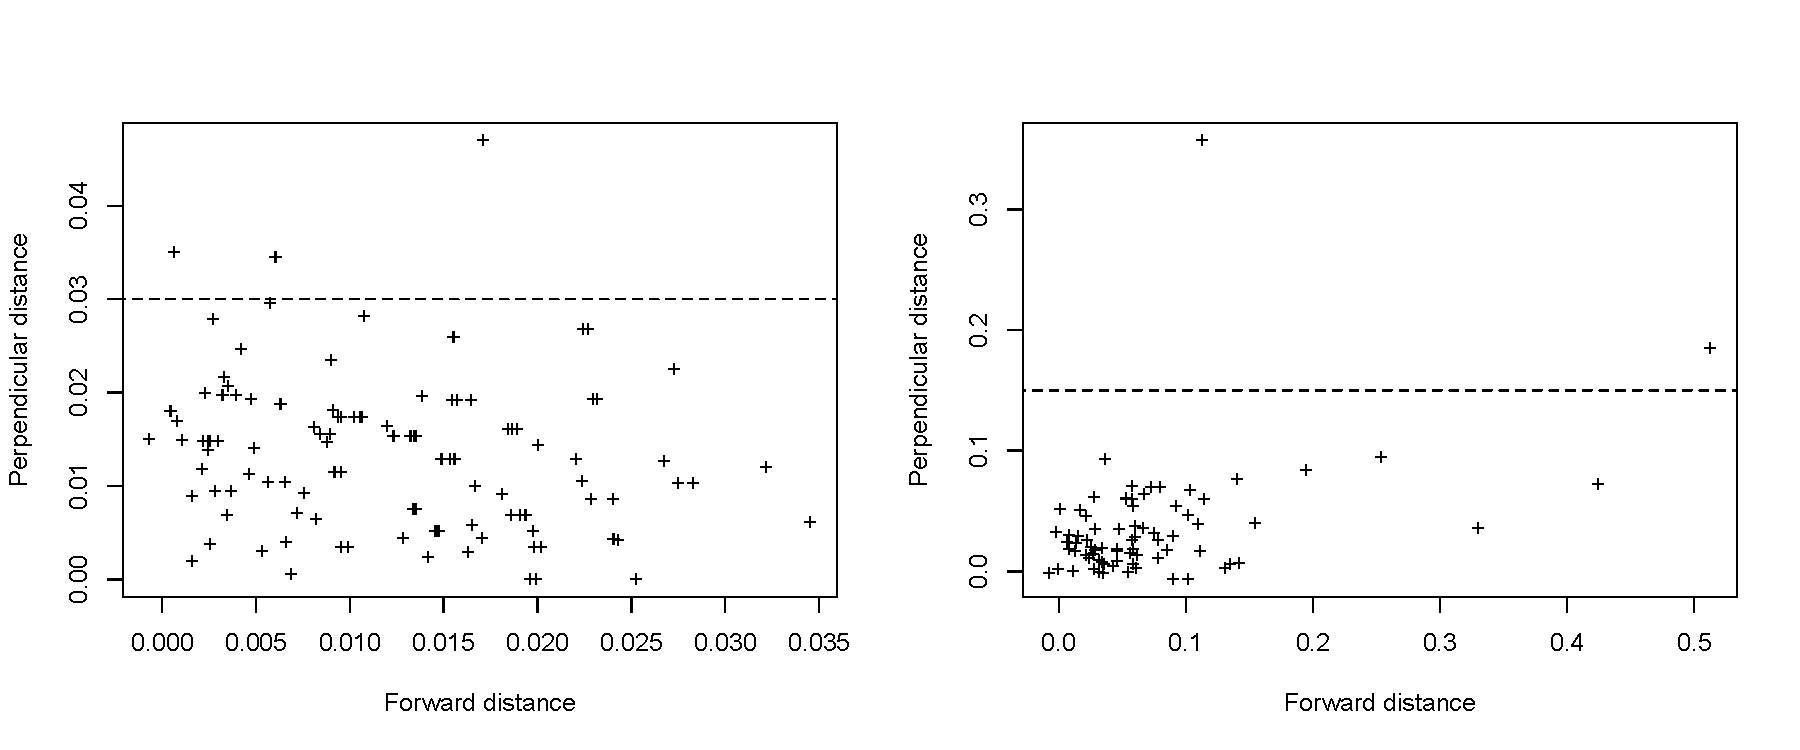
\includegraphics[scale=1]{Scatterplots.pdf}
\end{figure}

The first dataset has 127 detections of primates from a visual survey conducted by three sets of trained observers walking previously cut line transects in primary tropical rainforest at an elevation of 200-600m above sea level. The primates are believed to avoid the surveyors by moving some distance away from the paths, and the distribution of perpendicular distances of detected animals displays a mode at around 15m from the transect line (Figure~\ref{fig:primate.fits}).

\begin{figure}
\caption{Primate fits. The top row is perpendicular distance ($x$, in km) plots, the bottom forward distance ($y$, in km); the left column shows histograms and rug plots of observed data, with fitted PDFs (solid lines) overlaid, while the right column contains Q-Q plots. In the top left plot, the dashed line is the perpendicular distance detection function and the dotted line the animal distribution function $\pi(x;\boldsymbol{\phi})$. Circled points in the Q-Q plots show the points on which the Cramer-von Mises statistic is based. The bottom right Q-Q plot slopes down to reflect the fact that the CDF of forward distances is obtained by integrating time from 0 to $T$, which corresponds to integrating forward distance $y$ from right to left. The solid line in the bottom left plot is $E_x[f_{t|x}(t|x;\hat{\boldsymbol{\beta}})]$.\label{fig:primate.fits}}
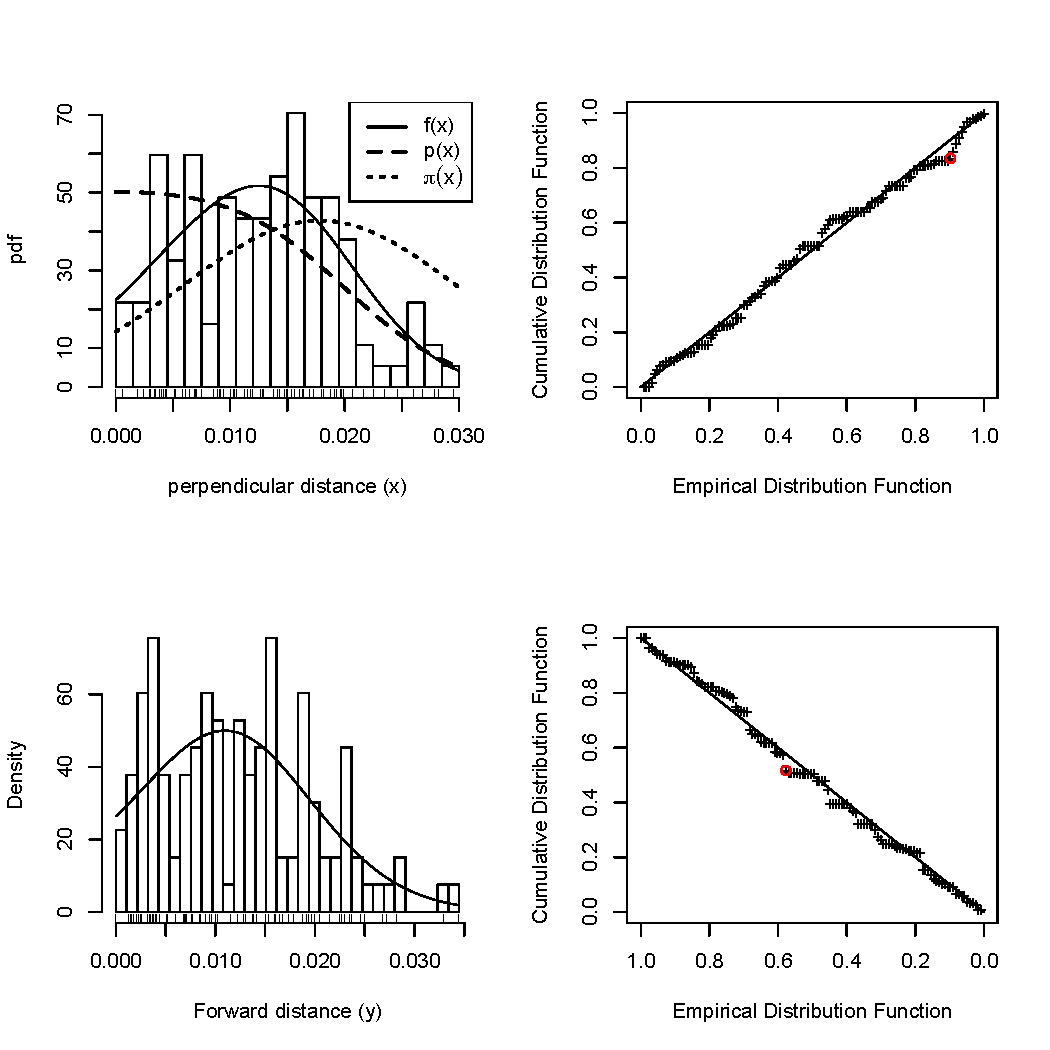
\includegraphics[scale=0.6]{PrimateFits.pdf}
\end{figure}

The second dataset has 76 detections of dolphin groups by one set of observers (the ``primary platform'') on a shipboard visual survey. This survey used two independent observers and data from both observers were analysed using mark-recapture distance sampling (MRDS) methods \cite[see][for an overview of these methods]{Burt+al:15} by \cite{Canadas+al:04}. They concluded that there was substantial attraction of schools towards the transect line. The perpendicular distance data have a mode at, or very close to distance zero (Figure~\ref{fig:dolphin.fits}).

\begin{figure}
\caption{Dolphin fits.  The top row is perpendicular distance ($x$, in km) plots, the bottom forward distance ($y$, in km); the left column shows histograms and rug plots of observed data, with fitted PDFs (solid lines) overlaid, while the right column contains Q-Q plots. In the top left plot, the dashed line is the perpendicular distance detection function and the dotted line the animal distribution function $\pi(x;\boldsymbol{\phi})$. Circled points in the Q-Q plots show the points on which the Cramer-von Mises statistic is based. The bottom right Q-Q plot slopes down to reflect the fact that the CDF of forward distances is obtained by integrating time from 0 to $T$, which corresponds to integrating forward distance $y$ from right to left. The solid line in the bottom left plot is $E_x[f_{t|x}(t|x;\hat{\boldsymbol{\beta}})]$.\label{fig:dolphin.fits}}
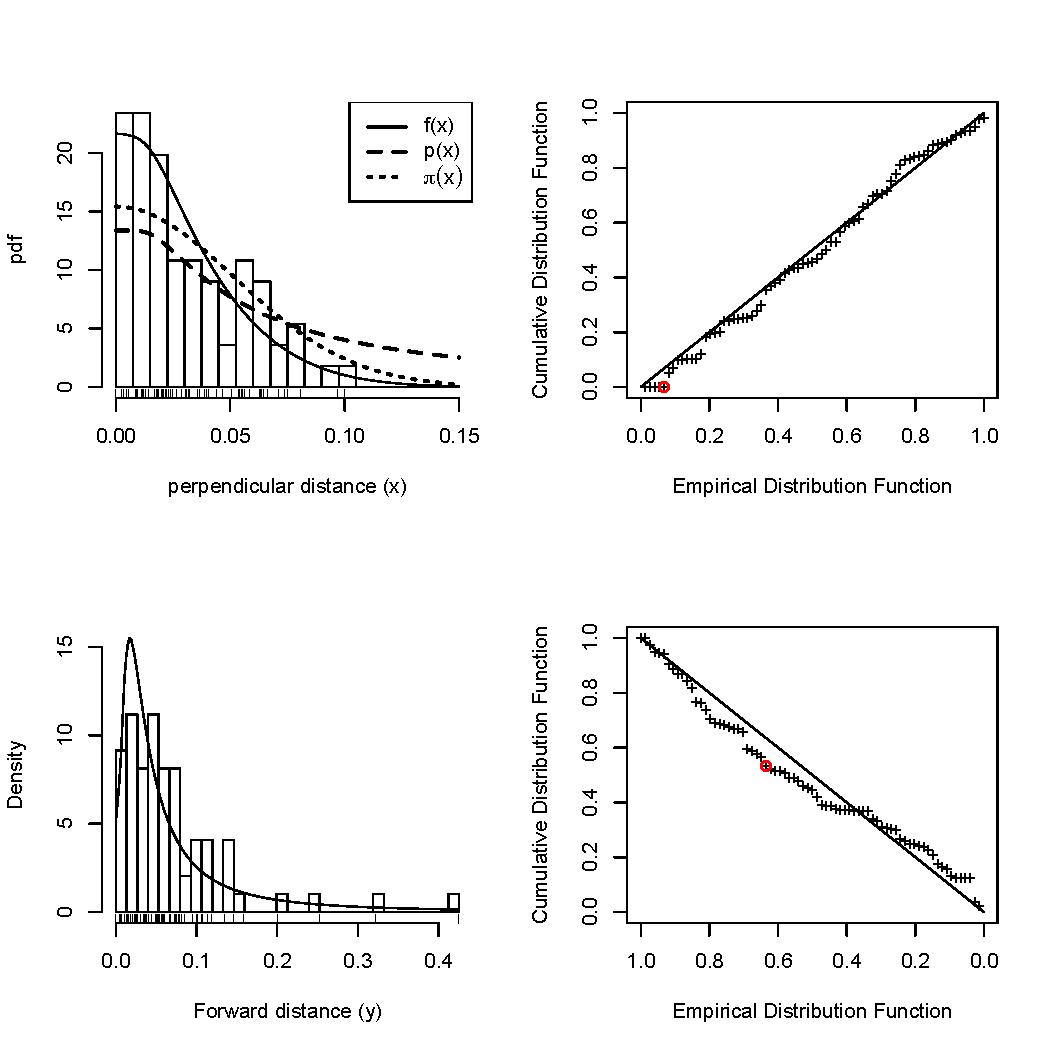
\includegraphics[scale=0.6]{DolphinFits.pdf}
\end{figure}

For each of these surveys, we estimate $\tilde{w}$ by maximising Equation~(\ref{eq:cond.lik}) and also by maximising the CDS likelihood, obtained by dropping $f_{t|s}(\boldmath{t}|\boldmath{s})$ from Equation~(\ref{eq:cond.lik}) and setting $\pi(x;\bmt{\phi})=C$ to reflect the CDS assumption that objects are distributed uniformly for $x\leq w$. CDS estimates were obtained using the \texttt{R} package  \texttt{Distance} \citep{Miller:15}.

\subsection{Primate survey results}

The primate data were truncated at perpendicular distance $w=0.03$ km, resulting in 4 detections being discarded. All models with $\pi_{U}$ had significantly bad fit in the $x$ dimension. Among models with non-significant goodness of fit statistics at the 5\% level, model pair $(h_{IP},\pi_{N})$ was selected on the basis of AIC, with the next best model $(h_{EP},\pi_{N})$ having an AIC larger by 8.6. However, parameters $\beta_2$ and $\beta_3$ of model $(h_{IP},\pi_{N})$ were found to be highly correlated (estimated correlation $>0.999$) and estimates from simulations using this model did not converge properly in 40\% of cases. We therefore fitted a reduced version of $(h_{IP},\pi_{N})$, which we call $(h_{IP0},\pi_{N})$, in which the scale parameter $\beta_2$ is fixed at 1. This resulted in a model with lower AIC than $(h_{IP},\pi_{N})$ and so we base inference on model $(h_{IP0},\pi_{N})$. (The point estimates of $\tilde{w}$ of these two models differ by less than 0.1\%) Goodness of fit tests give p-values of 0.72 (CvM)  and 0.63 (KS) in the $x$ dimension and 0.75 (CvM)  and 0.76 (KS) in the $y$ dimension. The fits of the chosen model in perpendicular and forward distance dimensions are shown in Figure~\ref{fig:primate.fits}. The chosen model has $p(0)=1$. 

A common, if ad-hoc way of dealing with data demonstrating avoidance of the transect lines, is to fit the hazard rate model of \cite{Hayes+Buckland:83} (which is equivalent to the 2D model $h_{HB}$ in the perpendicular distance dimension). This model has a flat shoulder and although it fits poorly to these data, the rationale for using it in the presence of avoidance is that it `undoes' the avoidance to some extent by averaging through the region from which animals have fled close to the line and to which they have fled farther from the line. This fitted model is shown in Figure~\ref{fig:CDSplots}. We also fitted the model $h_{HB}$ using the forward distance data (which CDS models do not use) in addition to perpendicular distance data, with $\pi_{U}$ (which is consistent with the CDS assumption of uniform animal density). This fitted model has an AIC that is larger by 54.9 than the preferred model $(h_{IP},\pi_{N})$. 

\begin{figure}
\caption{Conventional line transect hazard rate model fits. All distances are in kilometres. Primate data are on the left, dolphin data on the right. \label{fig:CDSplots}}
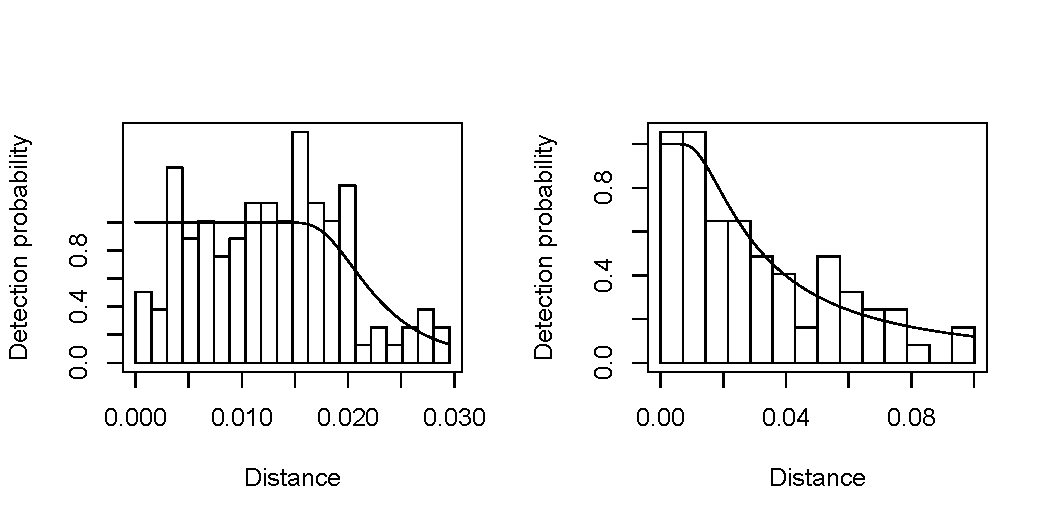
\includegraphics[scale=1]{CDSplots.pdf}
\end{figure}

The selected model $(h_{IP0},\pi_{N})$ has an estimated $\tilde{w}$ of 0.018 with a coefficient of variation (CV) of 12.5\% and 95\% confidence interval (CI) of (0.014, 0.023). The CDS model has an estimated $\tilde{w}$ 28\% larger at 0.023, with a CV of 5.8\%. Since estimated density is inversely proportional to $\tilde{w}$ (density is estimated as $\hat{D}=n/(2\widehat{\tilde{w}}L)$), the CDS model gives a density estimate that is some 22\% smaller than that from the selected 2D model.

The differences between the CDS estimate, which uses only perpendicular distance data and the estimates from our method, which uses 2D data (perpendicular and forward distances), are consistent with the CDS estimator not accounting adequately for the apparent avoidance of transect line by primates, and the 2D method accounting for the avoidance, albeit at the cost of additional variance due to estimating 2D hazard parameters and $\boldmath{\phi}$.

\subsection{Dolphin survey results}

The dolphin data were truncated at perpendicular distance $w=0.15$ km, resulting in two detections being discarded. Models were fitted to these data with distance distribution models $\pi_{U}$ and $\pi_{HN}$. All the models with $\pi_{U}$ had significantly bad fit. Among the models that did not have significantly bad fit, model $(h_{HB},\pi_{HN})$ was selected on the basis of AIC. All models that allow $p(0)<1$ had substantially worse AICs than model $(h_{HB},\pi_{HN})$. Goodness of fit tests give p-values for the selected model of 0.79  (CvM)  and 0.89 (KS) in the $x$ dimension and 0.24 (CvM)  and 0.42 (KS) in the $y$ dimension. The fits of the chosen model in perpendicular and forward distance dimensions is shown in Figure~\ref{fig:primate.fits}.
% * <martinjamescox@gmail.com> 2016-05-20T05:49:20.190Z:
%
% > km
%
% ^.

CDS methods were used to fit half-normal and hazard rate detection function models and the hazard rate model chosen by AIC. This fitted model is shown in Figure~\ref{fig:CDSplots}.

Model $(h_{HB},\pi_{N})$ has an estimated $\tilde{w}$ of 0.107 with a CV of 8.9\% and 95\% CI of (0.089, 0.127). The CDS model has an estimated $\tilde{w}$ some 40\% smaller at 0.064 with a CV of 18.8\%, generating a density estimate that is 67\% larger than that from model $(h_{HB},\pi_{N})$.

\cite{Canadas+al:04} obtained a density estimate of 0.123 schools per square nautical mile using MRDS methods that assume no unmodelled heterogeneity (no variables affecting detection probability of the two sets of observers that are not accounted for in the model). This will be a negatively biased estimate of density if there is unmodelled heterogeneity \citep[see][for a summary of this and related issues]{Burt+al:15}, and it is frequently the case that there is unmodelled heterogeneity on MRDS surveys. While there are ``point independence'' MRDS methods that relax the assumption of no unmodelled heterogeneity, these require uniform distribution of perpendicular distances of animals from the transect line and produce biased estimates in the presence of responsive movement \citep[see][]{Burt+al:15}. \cite{Canadas+al:04} also fitted a CDS model to the data and this produced an estimate of density 5.9 times larger than that from the MRDS method. The CDS estimate is positively biased in the presence of attraction to the transect line. Believing there to be attraction to the line, \cite{Canadas+al:04} chose what they believed to be the lesser of two evils and assumed no unmodelled heterogeneity (and hence a negatively biased estimate of density if unmodelled heterogeneity exists).

The estimated density from our method is 0.21 -- almost double the MRDS estimate and less than a third as big as the CDS estimate of \cite{Canadas+al:04}. This is consistent with the MRDS estimate being negatively biased (as is likely, due to unmodelled heterogeneity) and the CDS estimate being positively biased due to responsive movement. We do not claim that our estimator from model $(h_{HB},\pi_{HN})$ is unbiased in this case, because it seems quite likely that $p(0)$ is less than 1 \citep[][estimated it to be 0.79]{Canadas+al:04} due to animals being underwater some of the time. Although model $h_{HB}$ requires that $p(0)=1$, there are detections very close to $(x=0,y=0)$, as is evident from Figures~\ref{fig:Scatterplots} and detections at $(x=0,y=0)$ are consistent with $p(0)<1$. But sample size is small and this may give inadequate power to detect $p(0)<1$. In addition, the 2D method developed here assumes that $x$ does not change while animals are in view before they are detected, and this assumption may be violated for these data (although it is unclear how much this would bias estimates)

%\begin{figure}
%\caption{The mean estimated forward distance pdf (curve) and observed forward distance distribution (histogram) for the primate (left) and dolphin (right) detections that comprise the closest 10\% of detections to the transect line (no farther from the transect line than the dotted line shown in Figure~\ref{fig:Scatterplots}). If $p(0)$ is less than 1, the pdf has an intercept greater than zero. \label{fig:fy_x0fits}}
%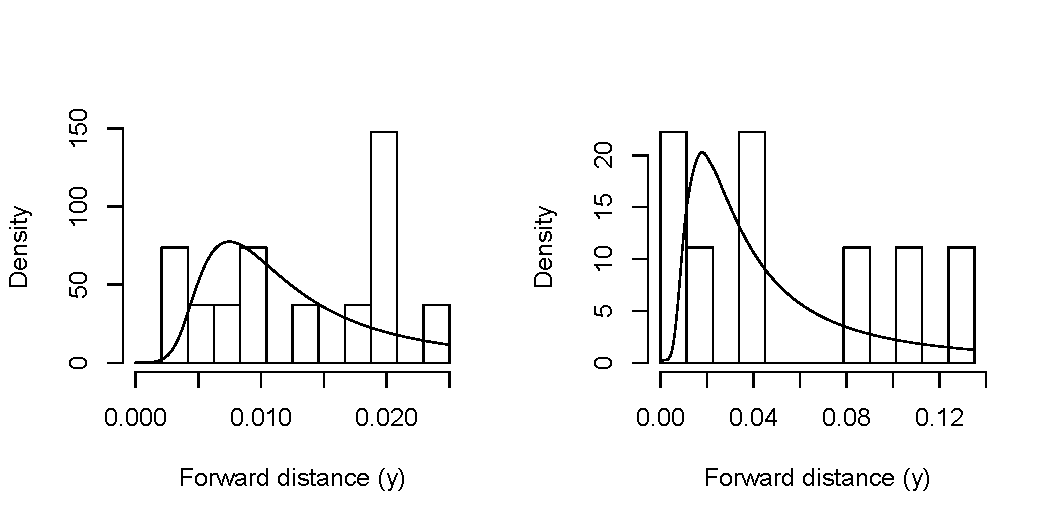
\includegraphics[scale=1]{fy_x0fits.pdf}
%\end{figure}

Nevertheless, as with the primate data analysis, the difference between the CDS estimate and the 2D method estimate is consistent with the 2D method being able to account for nonuniform distribution in the perpendicular distance dimension (attraction to the transect line in this case) and the CDS estimator not being able to do so.

We investigate by simulation below, the performance of the 2D method in the presence of unknown non-uniform animal distribution, and compare its performance to CDS estimators.


\section{Simulation study}

We consider two simulation scenarios: S1 treats the 2D model fitted to the primate data as truth, S2 treats the 2D model fitted to the dolphin data as truth with simulated data drawn from  $(h_{IP0},\pi_{N})$ in S1 and $(h_{HB},\pi_{HN})$ in S2. For all simulation scenarios we estimate $\tilde{w}$ using our 2D method and using a CDS estimator. We measure performance in terms of estimated $\tilde{w}$ relative bias and 95\% CI coverage probabilities. For each scenario we simulate 1,000 surveys, with each survey having a simulated sample size equal to that of the data sets, i.e. for simulation scenario S1 $n$ = 127, and simulation scenario S2 $n$ = 76. 

The 2D model estimator of $\tilde{w}$ is very nearly unbiased for S1 and unbiased for S2.  In both scenarios the 95\% confidence interval estimates have coverage close to their nominal level, while the CDS estimator has both substantial bias and very poor coverage probabilities (Table~\ref{tab:simResults}). 

In the case of the dolphin data, where it is likely that $p(0)$ is less than 1, we explored the ability of the 2D detection function models to estimate $p(0)$. To do this we simulated $(x,t)$ data from our fitted model ($h_{HB}$, $\pi_{HN}$) and then shifted the origin in the $t$ dimension forward (i.e reduced the time individuals are in view) until $p(0)$ was at a given value less than 1 (see below), and then fitted model ($h_{HB2}$, $\pi_{HN}$), which allows $p(0)<1$, to each of 1,000 simulated datasets. We did this for $p(0)\in\{0.9,0.8,0.7,0.6\}$. In all cases we foud $\hat{p}(0)$ to be negatively biased, with bias ranging from -12\% to -22\%. Although this is too small a simulation study to conclude that 2D detection function models are ineffective for $p(0)$ estimation, we would not recommend using them for this purpose without further investigation.

\begin{table}[ht]
%\centering
\caption{Simulation results for 2D and conventional distance sampling (CDS) estimation of effective strip half width ($\tilde{w}$), for simulations S1 (primates; avoidance) and S2 (dolphins; attraction). Coverage probability is the proportion of 95\% confidence interval estimates that contained the true $\tilde{w}$.} \label{tab:simResults}
\begin{tabular}{ccc}
  \hline
Simulation & mean percentage  & Coverage \\ 
Scenario  & relative bias & probability \\
  \hline
S1 2D  &  -2\% & 0.95 \\ 
S1 CDS &  37\% & 0.00 \\ 
S2 2D  &   0\% & 0.94 \\ 
S2 CDS & -39\% & 0.33 \\ 
   \hline
\end{tabular}
\end{table}



\section{Discussion and Conclusions}

We have shown that when animals are not distributed uniformly with respect to distance from the line on line transect surveys, unbiased estimates of $\tilde{w}$ can be obtained from 2D estimators that use forward distance or time to detection data as well as perpendicular distance, and that in such cases CDS estimators may be unreliable. The 2D estimators may be biased if there is responsive movement while within detectable range, but as the 2D model accommodates non-uniform distribution, it is likely that 2D estimators will be less biased than CDS estimators in this case.

%The ability of the 2D method estimators to deal with nonuniform distribution comes from using the information in forward detection distances (or times), which CDS methods neglect. 
We have also shown that use of forward detection distance data and 2D inference methods provides some information on whether the key CDS assumption that $p(0)=1$ has been violated. If $f_{t|x}(t=T|x=0;\hat{\boldsymbol{\beta}})=0$, this indicates that no objects ``survive'' detection at $x=0$, i.e. that $p(0)=1$. % (see Figure~\ref{fig:fy_x0fits} for example). 
Conversely, if $f_{t|x}(t=T|x=0;\hat{\boldsymbol{\beta}})$ is greater than zero, some animals avoid detection altogether and $p(0)<1$. In principle $p(0)$ can be estimated by $1-S(t=0,x;\hat{\boldsymbol{\beta}})$, where $\hat{\boldsymbol{\beta}}$ is the MLE of $\boldsymbol{\beta}$, but this should be done with care as small sample size may compromise the reliability of $p(0)$ estimation. The dolphin data are a case in point: it is likely from knowledge of the species and detection process, as well as from the analysis of \cite{Canadas+al:04}, that $p(0)<1$, and the histogram in Figure~\ref{fig:Scatterplots} % and \ref{fig:fy_x0fits} 
shows detections very close to zero forward and perpendicular distance, but the best model by AIC is one with $p(0)=1$. We consider the 2D method to be reliable when $p(0)$ is equal to, or close to 1, but it has limited ability to deal with $p(0)<1$. Recalling that the 2D line transect estimator can be seen as kind of removal method estimator, and that removal methods do not work well unless a large fraction of the population is removed, we believe these methods should be used with caution if $p(0)$ may be substantially less than 1.  With large enough sample size, inspection of the distribution of forward distances may be informative in this regard; if the distribution of forward distances of detections close to the line does not have a mode at $y>0$, this would suggest that $p(0)$ is less than 1.

We have not addressed the issue of how representative density within strips is of density overall when there in nonuniform animal distribution, and this is not something that can be inferred reliably from within-strip data alone. If strips are located randomly and nonuniformity is a consequence of responsive animal movement that does not involve any animals moving into or out of strips, then density within strips is representative of density outside strips. Nonuniform density can also arise from nonrandom placement of transects, even in the absence of responsive movement to observers. %(The CDS assumption of uniformity is usually justified on the basis of random transect placement.) 
In some cases it may be reasonable to use estimated density at the outer edge of strips as representative of density outside strips, but in general, drawing inferences about density outside strips from estimates of density in strips may be unreliable in the presence of nonuniform distribution within strips. \cite{Marques+al:10a} discuss these issues further.
% * <martinjamescox@gmail.com> 2016-05-20T05:51:34.058Z:
%
% > \cite{Marques+al:10a} discu
%
% ^.





We have not investigated use of times to detection with point transects. \cite{Marques+al:10a}, \cite{Cox+al:11} and \cite{Arranz+al:14} showed how radial distance and angle can be used to estimate density in the presence of nonuniform animal distribution. But if the gradient in detection probability with distance from observer coincides with gradient in density, then change in detection probability and change in density with distance are confounded even when detection angles are used. Time to detection data have the potential to deal with this. However, the methods of this paper assume that animals are stationary while within detectable distance and for most species, for any but very short survey times $T$, this is not a reasonable assumption for point transects. And with very short survey times, times to detection data are rather uninformative

The 2D detection function estimation method developed in this paper gives conservationists, managers, and others wanting to estimate animal abundance and density from line transect surveys a new tool for situations in which there is unknown object distribution within searched strips or circles. While it requires time to detection or (for line transects) forward distance at detection, these data are often quite easy to gather and we recommend that they be gathered as a matter of course where this is possible. 

%It is of course better to ensure that there is uniform animal distribution within the searched area, if this is possible, than to have to estimate this distribution. And in this case CDS estimators perform well.

Finally, we return to the question posed in the title of this paper: should distance sampling detection function models remain 1D or move to 2D? %When all CDS assumptions hold, CDS methods have a long history of performing well and we see no reason to move to 2D models in this case - although gathering time to detection or forward distance data for diagnostic purposes is still useful even then. 
Although time to detection data are in principle informative about $p(0)$, our limited simulations suggest that when $p(0)$ is not close to 1 and sample size is not large, estimation of $p(0)$ may not be reliable, and MRDS methods are probably preferable. An obvious extension of the methods of this paper would be the incorporation of time to detection data in MRDS models, but that is beyond the scope of this paper. On the other hand, we have shown the utility of 2D distance sampling data for line transect surveys when the CDS assumption that animals are uniformly distributed in the vicinity of observers is violated. We believe that unless the distribution of distances to individuals is known with confidence, distance sampling detection functions should be 2D, not 1D, as substantial bias can result from an incorrect assumption about the distribution. Moreover 2D detection functions can be used to investigate whether the observed data is consistent with an assumed distribution.  %We also note that 2D models are required to deal with stochastic animal availability; see \citep{Schweder:90}, \cite{Schweder+al:96}, \cite{Schweder+al:97}, \cite{Schweder+al:99}, \cite{Skaug+Schweder:99}, \cite{Okamura:03}, \cite{Skaug+al:04}, \cite{Okamura+al:03}, \cite{Okamura+al:06}, \cite{Okamura+al:12}, \cite{Borchers+al:13}, \cite{Langrock+al:13} and  \cite{Borchers+Langrock:ip}.

\section*{Supplementary Materials}

The \texttt{R} code and datasets used to do the analyses in this paper can be found on github at \href{https://github.com/david-borchers/LT2D}{https://github.com/david-borchers/LT2D} .

\section*{Acknowledgements}
We are grateful to Matthew Nowak from the Sumatran Orangutan Conservation Programme (SOCP) for allowing us to use the primate survey data from the Jantho Reintroduction Station. The initial survey was developed by Matthew Nowak and Serge Wich (Liverpool John Moores University) and then undertaken by the SOCP with funding from Chester Zoo. We are also grateful to the North Atlantic Marine Mammal Commission (NAMMCO) and the Faroese Museum of Natural History for allowing us to use the dolphin survey data from NASS95. MJC was funded by Australian Research Council grant FS110200057.

%\appendix
%\section{}
%\subsection{Any appendices necessary?}

\label{lastpage}

\bibliographystyle{biom}
\begin{thebibliography}{}

\bibitem[\protect\citeauthoryear{Amundson, Royle, and Handel}{Amundson
  et~al.}{2014}]{Amundson+al:14}
Amundson, C., J.~Royle, and C.~Handel (2014).
\newblock A hierarchical model combining distance sampling and time removal to
  estimate detection probability during avian point counts.
\newblock {\em The Auk\/}~{\em 131\/}(4), 476--494.

\bibitem[\protect\citeauthoryear{Arranz, Borchers, Aguilar~de Soto, Johnson,
  and Cox}{Arranz et~al.}{2014}]{Arranz+al:14}
Arranz, P., D.~L. Borchers, N.~Aguilar~de Soto, M.~P. Johnson, and M.~J. Cox
  (2014, April).
\newblock A new method to study inshore whale cue distribution from land-based
  observations.
\newblock {\em Marine Mammal Science\/}~{\em 30\/}(2), 810--818.

\bibitem[\protect\citeauthoryear{Borchers and Langrock}{Borchers and
  Langrock}{2015}]{Borchers+Langrock:ip}
Borchers, D. and R.~Langrock (2015).
\newblock Double-observer line transect surveys with markov-modulated poisson
  process models for animal availability.
\newblock {\em Biometrics\/}~{\em DOI: 10.1111/biom.12341}.

\bibitem[\protect\citeauthoryear{Borchers, Buckland, and Zucchini}{Borchers
  et~al.}{2002}]{Borchers+al:02}
Borchers, D.~L., S.~T. Buckland, and W.~Zucchini (2002).
\newblock {\em Estimating Animal Abundance: Closed Populations}.
\newblock Springer.

\bibitem[\protect\citeauthoryear{Borchers and Burnham}{Borchers and
  Burnham}{2004}]{Borchers+Burnham:04}
Borchers, D.~L. and K.~P. Burnham (2004).
\newblock General formulation for distance sampling.
\newblock In S.~T. Buckland, D.~R. Anderson, K.~P. Burnham, J.~L. Laake, D.~L.
  Borchers, and L.~J. Thomas (Eds.), {\em Advanced Distance Sampling.} Oxford
  University Press.

\bibitem[\protect\citeauthoryear{Borchers, Zucchini, Heide-Jorgensen, Canadas,
  and Langrock}{Borchers et~al.}{2013}]{Borchers+al:13}
Borchers, D.~L., W.~Zucchini, M.~P. Heide-Jorgensen, A.~Canadas, and
  R.~Langrock (2013).
\newblock Using hidden markov models to deal with availability bias on line
  transect surveys.
\newblock {\em Biometrics\/}~{\em 69}, 703--713.

\bibitem[\protect\citeauthoryear{Buckland, Oedekoven, and Borchers}{Buckland
  et~al.}{2015}]{Buckland+al:15}
Buckland, S., C.~Oedekoven, and D.~Borchers (2015).
\newblock Model-based distance sampling.
\newblock {\em Journal of Agricultural, Biological, and Environmental
  Statistics\/}, 1--18.

\bibitem[\protect\citeauthoryear{Buckland, Anderson, Burnham, Laake, Borchers,
  and Thomas}{Buckland et~al.}{2001}]{Buckland+al:01}
Buckland, S.~T., D.~R. Anderson, K.~P. Burnham, J.~L. Laake, D.~L. Borchers,
  and L.~J. Thomas (2001).
\newblock {\em Introduction to {D}istance {S}ampling}.
\newblock Oxford: Oxford University Press.

\bibitem[\protect\citeauthoryear{Buckland, Anderson, Burnham, Laake, Borchers,
  and Thomas}{Buckland et~al.}{2004}]{Buckland+al:04}
Buckland, S.~T., D.~R. Anderson, K.~P. Burnham, J.~L. Laake, D.~L. Borchers,
  and L.~J. Thomas (2004).
\newblock {\em Advanced {D}istance {S}ampling}.
\newblock Oxford: Oxford University Press.

\bibitem[\protect\citeauthoryear{Burnham}{Burnham}{1979}]{Burnham:79}
Burnham, K.~P. (1979).
\newblock A parametric generalization of the hayne estimator for line transect
  sampling.
\newblock {\em Biometrics\/}~{\em 35}, 587--595.

\bibitem[\protect\citeauthoryear{Burnham and Anderson}{Burnham and
  Anderson}{1976}]{Burnham+Anderson:76}
Burnham, K.~P. and D.~Anderson (1976).
\newblock Mathematical models for non-parametric inference from line transect
  data.
\newblock {\em Biometrics\/}~{\em 32}, 325--336.

\bibitem[\protect\citeauthoryear{Burt, Borchers, Jenkins, and Marques}{Burt
  et~al.}{2015}]{Burt+al:15}
Burt, M., D.~Borchers, K.~Jenkins, and T.~Marques (2015).
\newblock Using mark-recapture distance sampling methods on line transect
  surveys.
\newblock {\em Methods in Ecology and Evolution\/}~{\em 5}, 1180--1191.

\bibitem[\protect\citeauthoryear{Ca\~{n}adas, Desportes, and
  Borchers}{Ca\~{n}adas et~al.}{2004}]{Canadas+al:04}
Ca\~{n}adas, A., G.~Desportes, and D.~Borchers (2004).
\newblock The estimation of the detection function and g(0) for short-beaked
  common dolphins ({\em Delphinis delphis}), using double-platform data
  collected during the {NASS-95} {F}aroese survey.
\newblock {\em Journal of Cetacean Research and Management\/}~{\em 6},
  191--198.

\bibitem[\protect\citeauthoryear{Cox, Borchers, Demer, Cutter, and
  Brierley}{Cox et~al.}{2011}]{Cox+al:11}
Cox, M.~J., D.~L. Borchers, D.~A. Demer, G.~R. Cutter, and A.~S. Brierley
  (2011).
\newblock Estimating the density of antarctic krill ({\em Euphausia superba})
  from multi-beam echo-sounder observations using distance sampling methods.
\newblock {\em Journal of the Royal Statistical Society: Series C (Applied
  Statistics)\/}~{\em 60\/}(2), 301–316.

\bibitem[\protect\citeauthoryear{Eberhardt}{Eberhardt}{1978}]{Eberhardt:78}
Eberhardt, L. (1978).
\newblock Transect methods for population studies.
\newblock {\em Journal of Wildlife Management\/}~{\em 42}, 1--31.

\bibitem[\protect\citeauthoryear{Hayes and Buckland}{Hayes and
  Buckland}{1983}]{Hayes+Buckland:83}
Hayes, R.~J. and S.~T. Buckland (1983).
\newblock Radial-distance models for the line-transect method.
\newblock {\em Biometrics\/}~{\em 39}, 29--42.

\bibitem[\protect\citeauthoryear{Hayne}{Hayne}{1949}]{Hayne:49}
Hayne, D. (1949).
\newblock An examination of the strip census method for estimating animal
  populations.
\newblock {\em Journal of Wildlife Management\/}~{\em 13}, 145--157.

\bibitem[\protect\citeauthoryear{Langrock, Borchers, and Skaug}{Langrock
  et~al.}{2013}]{Langrock+al:13}
Langrock, R., D.~L. Borchers, and H.~J. Skaug (2013).
\newblock Markov-modulated nonhomogeneous poisson processes for modeling
  detections in surveys of marine mammal abundance.
\newblock {\em Journal of the Americal Statistical Association\/}~{\em 108},
  840--851.

\bibitem[\protect\citeauthoryear{Marques, Buckland, Borchers, Rexstad, and
  Thomas}{Marques et~al.}{2010}]{Marques+al:10}
Marques, T., S.~Buckland, D.~Borchers, E.~Rexstad, and L.~Thomas (2010).
\newblock Distance sampling.
\newblock In M.~Lovric (Ed.), {\em Springer's International Lexicon of
  Statistical Science}, pp.\  398--400. Springer.

\bibitem[\protect\citeauthoryear{Marques, Buckland, Borchers, Tosh, and
  McDonald}{Marques et~al.}{2010a}]{Marques+al:10a}
Marques, T.~A., S.~T. Buckland, D.~L. Borchers, D.~Tosh, and R.~A. McDonald
  (2010a).
\newblock Point transect sampling along linear features.
\newblock {\em Biometrics\/}~{\em 66\/}, 1247--1255.

\bibitem[\protect\citeauthoryear{Miller}{Miller}{2015}]{Miller:15}
Miller, D.~L. (2015).
\newblock {\em Distance: Distance Sampling Detection Function and Abundance
  Estimation}.
\newblock R package version 0.9.4.

\bibitem[\protect\citeauthoryear{Oehlert}{Oehlert}{1992}]{Oehlert:92}
Oehlert, D. (1992).
\newblock A note on the delta method.
\newblock {\em The American Statistician\/}~{\em 46\/}, 27--29.

\bibitem[\protect\citeauthoryear{Okamura}{Okamura}{2003}]{Okamura:03}
Okamura, H. (2003).
\newblock A line transect method to estimate abundance of long-diving animals.
\newblock {\em Fisheries Science\/}~{\em 69}, 1176--1181.

\bibitem[\protect\citeauthoryear{Okamura, Kitakado, Hiramatsu, and
  Mori}{Okamura et~al.}{2003}]{Okamura+al:03}
Okamura, H., T.~Kitakado, K.~Hiramatsu, and M.~Mori (2003).
\newblock Abundance estimation of diving animals by the double-platform line
  transect method.
\newblock {\em Biometrics\/}~{\em 59}, 512--520.

\bibitem[\protect\citeauthoryear{Okamura, Minamakawa, and Kitakado}{Okamura
  et~al.}{2006}]{Okamura+al:06}
Okamura, H., S.~Minamakawa, and T.~Kitakado (2006).
\newblock Effect of surfacing patterns on abundance estimates of long-diving
  animals.
\newblock {\em Fisheries Science\/}~{\em 72}, 631--638.

\bibitem[\protect\citeauthoryear{Okamura, Minamikawa, Skaug, and
  Kishiro}{Okamura et~al.}{2012}]{Okamura+al:12}
Okamura, H., S.~Minamikawa, H.~J. Skaug, and T.~Kishiro (2012).
\newblock Abundance estimation of long-diving animals using line transect
  methods.
\newblock {\em Biometrics\/}~{\em 68}, 504--513.

\bibitem[\protect\citeauthoryear{Schweder}{Schweder}{1974}]{Schweder:74}
Schweder, T. (1974).
\newblock {\em Transformations of point processes: applications to animal
  sighting and catch problems, with special emphasis on whales}.
\newblock Ph{D} thesis, University of California, Berkeley.

\bibitem[\protect\citeauthoryear{Schweder}{Schweder}{1990}]{Schweder:90}
Schweder, T. (1990).
\newblock Independent observer experiments to estimate the detection function
  in line transect surveys of whales.
\newblock {\em Report of the International Whaling Commission\/}~{\em 40},
  349--356.

\bibitem[\protect\citeauthoryear{Schweder, Hagen, Helgeland, and
  Koppervik}{Schweder et~al.}{1996}]{Schweder+al:96}
Schweder, T., G.~Hagen, J.~Helgeland, and I.~Koppervik (1996).
\newblock Abundance estimation of northeastern {A}tlantic minke whales.
\newblock {\em Report of the International Whaling Commission\/}~{\em 46},
  391--405.

\bibitem[\protect\citeauthoryear{Schweder, Skaug, Dimakos, Langaas, and
  Oien}{Schweder et~al.}{1997}]{Schweder+al:97}
Schweder, T., H.~J. Skaug, X.~K. Dimakos, M.~Langaas, and N.~Oien (1997).
\newblock Abundance of northeastern {A}tlantic minke whale, estimates for 1989
  and 1995.
\newblock {\em Report of the International Whaling Commission\/}~{\em 47},
  453--483.

\bibitem[\protect\citeauthoryear{Schweder, Skaug, Langaas, and
  Dimakos}{Schweder et~al.}{1999}]{Schweder+al:99}
Schweder, T., H.~J. Skaug, M.~Langaas, and X.~K. Dimakos (1999).
\newblock Simulated likelihood methods for complex double-platform line
  transect surveys.
\newblock {\em Biometrics\/}~{\em 55}, 678--687.

\bibitem[\protect\citeauthoryear{Seber}{Seber}{1982}]{Seber:82}
Seber, G. A.~F. (1982).
\newblock {\em The estimation of animal abundance and related parameters\/}
  (2nd ed.).
\newblock London: Charles Griffin.

\bibitem[\protect\citeauthoryear{Skaug and Schweder}{Skaug and
  Schweder}{1999}]{Skaug+Schweder:99}
Skaug, H. and T.~Schweder (1999).
\newblock Hazard models for line transect surveys with independent observers.
\newblock {\em Biometrics\/}~{\em 55}, 29--36.

\bibitem[\protect\citeauthoryear{Skaug, Oien, Schweder, and Bothun}{Skaug
  et~al.}{2004}]{Skaug+al:04}
Skaug, H.~J., N.~Oien, T.~Schweder, and F.~G. Bothun (2004).
\newblock Current abundance of minke whales ({\em Balaenoptera acutorostrata})
  in the northeast atlantic; variability in time and space.
\newblock {\em Canadian Journal of Fisheries and Aquatic Sciences\/}~{\em 61},
  870--886.

\bibitem[\protect\citeauthoryear{Solymos, Matsuoka, Bayne, Lele, Fontaine,
  Cumming, Stralberg, Schmiegelow, and Song}{Solymos
  et~al.}{2013}]{Solymos+al:13}
Solymos, P., S.~Matsuoka, E.~Bayne, S.~Lele, P.~Fontaine, S.~Cumming,
  D.~Stralberg, F.~Schmiegelow, and S.~Song (2013).
\newblock Calibrating indices of avian density from non-standardized survey
  data: making the most of a messy situation.
\newblock {\em Methods in Ecology and Evolution\/}~{\em 4\/}(11), 1047--1058.

\end{thebibliography}
\end{document}